\chapter{Descripción del Trabajo}
\label{cap:descripcionTrabajo}

Aquí comienza la descripción del trabajo realizado. Se deben incluir tantos capítulos como sea necesario para describir de la manera más completa posible el trabajo que se ha llevado a cabo. Como muestra la figura \ref{fig:sampleImage}, está todo por hacer.

\begin{figure}[h]
	\centering
	
\includegraphics[width = 0.5\textwidth]{Imagenes/Vectorial/Todo.pdf}
	\caption{Ejemplo de imagen}
	\label{fig:sampleImage}
\end{figure}

Si te sirve de utilidad,  puedes incluir tablas para mostrar resultados, tal como se ve en la tabla \ref{tab:sampleTable}.


\begin{table}[h]
	\centering
	\begin{tabular}{c|c|c}
		\textbf{Col 1} & \textbf{Col 2} & \textbf{Col 3} \\
		\hline\hline
		3 & 3.01 & 3.50\\
		6 & 2.12 & 4.40\\
		1 & 3.79 & 5.00\\
		2 & 4.88 & 5.30\\
		4 & 3.50 & 2.90\\
		5 & 7.40 & 4.70\\
		\hline
	\end{tabular}
	\caption{Tabla de ejemplo}
	\label{tab:sampleTable}
\end{table}

\section{Explicaciones}

Una vez tengamos las consultas básicas, crearemos otras más complejas que devuelvan información útil para relacionar canciones. Estudiaremos estas consultas con el objetivo de establecer un número de explicaciones que determinen si una canción podría estar relacionada con otra.

En una primera fase, buscaremos explicaciones básicas para relacionar diferentes tipos de canciones, por ejemplo: género, artista, álbum, etc. Después buscaremos explicaciones más complejas que normalmente un humano pasaría por alto. Asignaremos una complejidad de k=1 a las explicaciones básicas. Estas explicaciones son una relación directa entre dos canciones relacionadas por una propiedad.\\

(DRAW)\\

Las explicaciones complejas, sin embargo, pueden estar formadas por relaciones indirectas entre los datos de una forma que se puede representar con un grafo. Estas explicaciones pueden tener un nivel de complejidad diferente (k= 2, 3, 4...) dependiendo de cuántas aristas del grafo separen ambos elementos.\\

(DRAW)\\


\subsection{Explicaciones directas}

\subsubsection*{Popularidad}

Una de las principales explicaciones que debemos contemplar es la popularidad de las canciones. En un dataset hay unas canciones que son más escuchadas que otras. Es útil tomar ese punto en consideración cuando necesitemos recomendar una canción basándonos en la idea de que las canciones populares tendrán una mayor probabilidad de encajar con otras. Por ejemplo, si tenemos que recomendar una canción pop será una mejor elección un tema de Michael Jackson, uno de los artistas más representativos del género, antes que recomendar una canción o artista poco popular.

\subsubsection*{Artista}

El artista es una de las explicaciones más obvias pero también es una de las más importantes. Esta explicación hace referencia a cuando dos temas son interpretadas por el mismo artista, por lo que tienen una clara relación directa ya que suele existir similitud entre las canciones de un artista.

Como ejemplo podemos tomar los temas \textit{One More Time} y \textit{Get Lucky}. Ambos son interpretados por el dúo musical \textbf{Daft Punk}, así que podemos explicar su relación gracias a este dato.

Para esta explicación utilizamos la propiedad ``performer'' (intérprete) de Wikidata. Siguiendo el modelo RDF, el sujeto es la canción (\textit{One More Time}, por ejemplo), el predicado es la propiedad intérprete y el objeto es el artista (\textbf{Daft Punk}). \\

\begin{figure}[h!]
	\centering
	
\includegraphics[width = 0.9\textwidth]{Imagenes/Bitmap/Artista ejemplo.png}
	\caption{Ejemplo de explicación por artista}
	\label{fig:sampleImage}
\end{figure}

\subsubsection*{Álbum}

Una explicación muy potente será que ambas canciones pertenezcan al mismo álbum. A menudo esta explicación aparecerá acompañada de la explicación del artista y, en cualquier caso, la relación que existe entre dos temas del mismo álbum suele ser más estrecha debido a que poseen más puntos en común, como puede ser el género, la fecha o la temática.

Tomemos como ejemplo \textit{Smells Like Teen Spirit} y \textit{Come as You Are}. Estas dos canciones son muy cercanas porque tienen varios puntos en común, pero una de las explicaciones que podemos ofrecer es que ambas pertenecen al álbum \textit{Nevermind}, de \textbf{Nirvana}. \textit{About a Girl} es otro tema que se podría recomendar a raíz de \textit{Smells Like Teen Spirit}, pero es una peor elección que \textit{Come as You Are} porque pertenece a un álbum diferente.

Volvemos a utilizar Wikidata para obtener esta explicación, concretamente la propiedad ``part of'' (parte de). Esta propiedad se utiliza para varias cosas, entre ellas indicar los álbumes a los que pertenecen las canciones. Así obtenemos que \textit{Smells Like Teen Spirit} es ``parte de'' \textit{Nevermind}.\\

\begin{figure}[h!]
	\centering
	
\includegraphics[width = 0.9\textwidth]{Imagenes/Bitmap/Álbum ejemplo.png}
	\caption{Ejemplo de explicación por álbum}
	\label{fig:sampleImage}
\end{figure}

\subsubsection*{Década}

Creemos que hay una mayor probabilidad de que exista una relación entre dos canciones que pertenezcan a la misma década. Esto se debe a que a lo largo del tiempo ha habido periodos marcados por uno o varios géneros musicales. Esto también ayuda a estudiar cómo estos distintos géneros están relacionados entre sí, lo cual es otro punto importante a tener en cuenta ya que hay géneros íntimamente relacionados entre sí: techno y house, heavy metal y thrash metal, etc.

Gracias a esta explicación, podemos relacionar dos canciones que a priori son muy distintas, como es el caso de \textit{September} de \textbf{Earth, Wind \& Fire} y \textit{Bohemian Rhapsody} de \textbf{Queen}. Estos temas no comparten algo tan básico como el artista o el género, pero ambos fueron publicados en los años 70 y por ello pueden resultar interesantes para un usuario que busque escuchar los ritmos de esa época.

Para obtener esta explicación, emplearemos la propiedad ``publication date'' (fecha de publicación) de las canciones en Wikidata y comprobaremos si las dos fechas se sitúan dentro de la misma década.\\

\begin{figure}[h!]
	\centering
	\includegraphics[width = 0.9\textwidth]{Imagenes/Bitmap/Década ejemplo.png}
	\caption{Ejemplo de explicación por década}
	\label{fig:sampleImage}
\end{figure}

\subsubsection*{Premios}

La siguiente explicación son los premios recibidos. Existe una variedad de premios compartidos por diferentes canciones. Algunos de estos premios son más específicos que otros, pero en cualquier caso pueden resultar una relación útil para el recomendador ya que son un reflejo de la repercusión de las canciones. Nuestro objetivo es encontrar al menos un premio que hayan recibido ambas canciones.

Así explicaríamos la relación entre \textit{Single Ladies (Put a Ring on It)} de \textbf{Beyoncé} y \textit{Rolling in the Deep} de \textbf{Adele}, ya que ambos temas han recibido el Premio Grammy a la canción del año.

Usaremos la propiedad ``award received'' (premio recibido) encontrada en Wikidata. De esta forma, \textit{Rolling in the Deep} sería el sujeto, ``award received'' sería el predicado y \textit{Grammy Award for Song of the Year} sería el objeto.\\

\begin{figure}[h!]
	\centering
	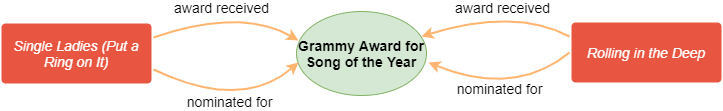
\includegraphics[width = 0.9\textwidth]{Imagenes/Bitmap/Premio ejemplo.png}
	\caption{Ejemplo de explicación por premio}
	\label{fig:sampleImage}
\end{figure}

\subsubsection*{Género}

La explicación Género es una de las más representativas ya que las personas se guían por el género que prefieren para escuchar canciones similares, aunque en ocasiones no deba ser así. Un usuario que sea fan del jazz querrá escuchar canciones de ese mismo género o géneros similares porque todas los temas de un mismo género comparten una serie de puntos en común como la elección de los instrumentos, temáticas similares en sus letras o patrones de composición.

Gracias al género, podemos explicar la relación entre canciones como \textit{Master of Puppets} de \textbf{Metallica} e \textit{Indians} de \textbf{Anthrax}, que pertenecen al \textbf{thrash metal}.

Para esta relación utilizamos la propiedad ``genre'' (género) de Wikidata. Así tenemos que la canción \textit{Master of Puppets} pertenece al género \textbf{thrash metal}.\\

\begin{figure}[h!]
	\centering
	\includegraphics[width = 0.9\textwidth]{Imagenes/Bitmap/Género ejemplo.png}
	\caption{Ejemplo de explicación por género}
	\label{fig:sampleImage}
\end{figure}

Además, si hacemos un estudio más profundo de los géneros y la frecuencia en que aparecen juntos dentro de las mismas canciones, podemos llegar a relacionar temas de géneros que no son idénticos en nuestra fuente pero sí similares. Este sería el caso de \textit{Fight the Power} de \textbf{Public Enemy} y \textit{Juicy} de \textbf{The Notorious B.I.G.}, siendo el primero considerado un tema de \textbf{hip hop music} según la información de Wikidata mientras que el segundo aparece como \textbf{political hip hop}.

\subsubsection*{Compañía discográfica}

Compañía discográfica hace referencia a la compañía por la que ha firmado el artista para publicar un tema concreto. Hemos podido observar que una misma compañía puede firmar a artistas que a veces no tienen relación ninguna en cuanto al estilo musical, pero hay otras causas que sí los pueden relacionar indirectamente como la tendencia del momento, el target del público que generan, etc.

Para ilustrarlo con un ejemplo, tanto la canción \textit{Born in the U.S.A.} de \textbf{Bruce Springsteen} como la canción \textit{Ashes} de \textbf{Céline Dion} fueron publicadas por el sello discográfico \textbf{Columbia Records}.

Podemos alcanzar esta explicación gracias a la propiedad ``record label'' (sello discográfico) de Wikidata. \textit{Born in the U.S.A.} tiene un ``record label'' cuyo nombre (o valor) es \textbf{Columbia Records}.\\

\begin{figure}[h!]
	\centering
	\includegraphics[width = 0.9\textwidth]{Imagenes/Bitmap/Discográfica ejemplo.png}
	\caption{Ejemplo de explicación por compañía discográfica}
	\label{fig:sampleImage}
\end{figure}

\subsubsection*{Singles}

Existe también una cierta relación entre aquellos temas que sean singles o sencillos, así que consideramos esto como una explicación más. El razonamiento para esta decisión es que los singles son canciones que se publican de forma independiente por razones promocionales, por lo que suelen convertirse en los temas más populares y representativos del trabajo del artista. Por ello, pueden poseer más valor para el recomendador que otras canciones porque los singles tienen más probabilidades de coincidir con los gustos del usuario.

El tema \textit{Bad Guy} de \textbf{Billie Eilish} es un single, así que podemos decir que tiene cierta relación con \textit{Shallow} de \textbf{Lady Gaga} y \textbf{Bradley Cooper}, que también es un single.

Para esta explicación emplearemos la propiedad ``instance of'' (instancia de) en Wikidata y su valor ``single''. De esta forma comprobaremos que tanto \textit{Bad Guy} como \textit{Shallow} son ``instancia de'' ``single''.\\

\begin{figure}[h!]
	\centering
	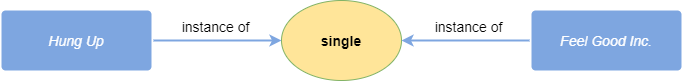
\includegraphics[width = 0.9\textwidth]{Imagenes/Bitmap/Single ejemplo.png}
	\caption{Ejemplo de explicación por single}
	\label{fig:sampleImage}
\end{figure}

\subsection{Explicaciones indirectas}

La explicaciones indirectas nos van a ofrecer relaciones más complejas que nos proporcionen información que a simple vista no podríamos relacionar.
El principal método que hemos establecido es proseguir el estudio de las explicaciones directas creando un grafo en forma de árbol.
Para cada una de las explicaciones directas ejecutaremos más consultas SPARQL obteniendo\\


A continuación enumeramos las explicaciones indirectas adicionales que buscamos para establecer la relación entre dos canciones:

\subsubsection*{País de origen}

Para empezar podemos fijarnos en el país de origen de los artistas. Esta explicación puede ser especialmente útil para países relativamente pequeños donde la música nacional presenta unos patrones claros. Además, a lo largo de la historia en un país se genera una tendencia o nuevo género musical el cual es propio de ese país.

La canción \textit{Fire} de la banda \textbf{BTS} y \textit{Kill This Love} de \textbf{Blackpink} guardan cierta similitud porque ambos grupos son originarios de \textbf{Corea del Sur}.

Para comprobarlo, primero tendremos que usar la propiedad de Wikidata ``performer'', como ya hicimos en la explicación del Artista, y después comprobar la propiedad ``country of origin'' (país de origen) en el caso de las bandas o la propiedad ``country of citizenship'' (país de nacionalidad) en el caso de los artistas en solitario. \textit{Fire} tiene el ``performer'' \textbf{BTS}, cuyo ``country of origin'' es Corea del Sur.

\subsubsection*{Banda sonora}

También es interesante comprobar si ambas canciones aparecen en la \textbf{banda sonora} de una misma película. Para esta explicación necesitaremos recurrir a una fuente como MusicBrainz debido a que la información de Wikidata es insuficiente en lo referente a bandas sonoras.

\subsubsection*{Influencia}

La \textbf{influencia de los artistas} es otra explicación importante. A menudo el trabajo de un artista se ve influenciado por otros artistas de formas que no siempre están ligadas a un género musical concreto, así que podemos encontrar una relación entre dos canciones examinando estas influencias.

Tomando como ejemplo las canciones \textit{Billie Jean} de \textbf{Michael Jackson} y \textit{Paint It Black} de \textit{The Rolling Stones}, podemos establecer una relación entre ellas al ver que ambos artistas fueron influenciados por la banda \textbf{The Beatles}.

Obtenemos esta explicación gracias a la propiedad ``influenced by'' (influenciado por) de Wikidata, además de la propiedad ``performer'' para relacionar el tema con su artista. Así averiguamos que \textit{Billie Jean} tiene de ``intérprete'' a \textbf{Michael Jackson}, quien fue ``influenciado por'' \textbf{The Beatles}.

\subsubsection*{Integrantes}

De la misma forma, un artista puede pertenecer a dos o más bandas musicales a lo largo de su carrera. Comparando \textbf{los integrantes de las bandas} podemos encontrar otra explicación para relacionar dos canciones entre sí, ya que esta presencia de un mismo artista en diferentes proyectos suele influir al sonido de los mismos. Además, los aficionados de un artista concreto a menudo desean escucharlo en todas las etapas de su carrera musical.

Si tomamos los temas \textit{Lithium} de \textbf{Nirvana} y \textit{The Pretender} de \textbf{Foo Fighters} podemos observar que existe una relación entre ellos porque el músico \textbf{Dave Grohl} ha formado parte de ambas bandas.

Para comprobarlo usaremos la propiedad de Wikidata ``performer'' y después comprobaremos la propiedad ``has part'' (formado por) para ver todos los miembros de la banda y buscar coincidencias. De este modo, podemos ver que \textit{The Pretender} tiene un ``performer'' que es \textbf{Foo Fighters}, y a su vez \textbf{Foo Fighters} ``has part'' \textbf{Dave Grohl}.

\subsubsection*{Tipo de voz}

Siguiendo con el estudio de los artistas, el \textbf{tipo de voz} de los vocalistas es una buena explicación para relacionar dos canciones. El tipo de voz influye en el sonido general del tema y puede ser especialmente determinante en ciertos géneros musicales. Por limitaciones técnicas, solo aplicaremos esta explicación con artistas en solitario.

La voz de un artista puede encajar en más de un tipo, como veremos en el siguiente ejemplo, aunque en esta explicación buscamos que coincidan en al menos un tipo. La cantante \textbf{Lady Gaga} se asemeja a \textbf{Amy Winehouse} por su tipo de voz, ya que ambas son \textit{mezzo-soprano} y \textit{contralto}. Así podemos explicar la relación entre dos canciones de estas artistas como \textit{Poker Face} y \textit{Rehab}.

Para esta explicación resulta útil la propiedad ``voice type'' (tipo de voz) en Wikidata. Partiendo de \textit{Poker Face}, utilizamos la propiedad ``performer'' para llegar a \textbf{Lady Gaga} y finalmente usamos su ``voice type'' para obtener \textit{mezzo-soprano}.